\documentclass[a4paper,10pt]{article}
\usepackage[utf8]{inputenc}
\usepackage[a4paper,
            bindingoffset=0.2in,
            left=1in,
            right=1in,
            top=1in,
            bottom=1in,
            footskip=.25in]{geometry}

%###############################################################################

%\input{~/layout/global_layout}


%###############################################################################

% packages begin

\usepackage[
  backend=biber,
  sortcites=true,
  style=alphabetic,
  eprint=true,
  backref=true
]{biblatex}
\addbibresource{bibliographie.bib}
\usepackage[acronym]{glossaries}

\usepackage{euscript}[mathcal]
% e.g. \mathcal{A} for fancy letters in mathmode
\usepackage{amsmath,amssymb,amstext,amsthm}

\usepackage{mdframed}
\newmdtheoremenv[nobreak=true]{problem}{Problem}[subsection]
\newmdtheoremenv[nobreak=true]{claim}{Claim}[subsection]
\newtheorem{definition}{Definition}[subsection]
\newtheorem{lemma}{Lemma}[claim]
\newtheorem{plemma}{Lemma}[problem]

\usepackage{mathtools}
\DeclarePairedDelimiter\ceil{\lceil}{\rceil}
\DeclarePairedDelimiter\floor{\lfloor}{\rfloor}

\usepackage{enumerate}
\usepackage[pdftex]{graphicx}
\usepackage{subcaption}
% 'draft' für schnelleres rendern mitübergeben -> [pdftex, draft]
% dadruch wird nicht das bild mitgerendered, sondern nur ein kasten mit bildname -> schont ressourcen

\usepackage{hyperref}

\usepackage{tikz}
\usetikzlibrary{arrows,automata,matrix,positioning,shapes}

% for adding non-formatted text to include source-code
\usepackage{listings}
\lstset{language=Python,basicstyle=\footnotesize}
% z.B.:
% \lstinputlisting{source_filename.py}
% \lstinputlisting[lanugage=Python, firstline=37, lastline=45]{source_filename.py}
%
% oder
%
% \begin{lstlisting}[frame=single]
% CODE HERE
%\end{lstlisting}
\usepackage{algorithm}
\usepackage{algpseudocode}

\usepackage{wasysym}

\usepackage{titling}
\usepackage{titlesec}
\usepackage[nocheck]{fancyhdr}
\usepackage{lastpage}

\usepackage{kantlipsum}
\usepackage[colorinlistoftodos,prependcaption,textsize=tiny]{todonotes}

% packages end
%###############################################################################

\pretitle{% add some rules
  \begin{center}
    \LARGE\bfseries
} %, make the fonts bigger, make the title (only) bold
\posttitle{%
  \end{center}%
  %\vskip .75em plus .25em minus .25em% increase the vertical spacing a bit, make this particular glue stretchier
}
\predate{%
  \begin{center}
    \normalsize
}
\postdate{%
  \end{center}%
}

\titleformat*{\section}{\Large\bfseries}
\titleformat*{\subsection}{\large\bfseries}
\titleformat*{\subsubsection}{\normalsize\bfseries}

\titleformat*{\paragraph}{\Large\bfseries}
\titleformat*{\subparagraph}{\large\bfseries}

%###############################################################################

\pagestyle{fancy}
\fancyhf{}
% l=left, c=center, r=right; e=even_pagenumber, o=odd_pagenumber; h=header, f=footer
% example: [lh] -> left header, [lof,ref] -> fotter left when odd, right when even
%\fancyhf[lh]{}
%\fancyhf[ch]{}
%\fancyhf[rh]{}
%\fancyhf[lf]{}
\fancyhf[cf]{\footnotesize Page \thepage\ of \pageref*{LastPage}}
%\fancyhf[rf]{}
\renewcommand{\headrule}{} % removes horizontal header line

% Fotter options for first page

\fancypagestyle{firstpagestyle}{
  \renewcommand{\thedate}{\textmd{}} % removes horizontal header line
  \fancyhf{}
  \fancyhf[lh]{\ttfamily M.Sc. Computer Science\\KTH Royal Institute of Technology}
  \fancyhf[rh]{\ttfamily Period 4\\\today}
  \fancyfoot[C]{\footnotesize Page \thepage\ of \pageref*{LastPage}}
  \renewcommand{\headrule}{} % removes horizontal header line
}
%###############################################################################

\newcommand\extrafootertext[1]{%
    \bgroup
    \renewcommand\thefootnote{\fnsymbol{footnote}}%
    \renewcommand\thempfootnote{\fnsymbol{mpfootnote}}%
    \footnotetext[0]{#1}%
    \egroup
}

%###############################################################################

\title{
  \normalsize{DD2356 VT25 Methods in}\\
  \normalsize{High Performance Computing}\\
  \large{Assignment 4}
}
\author{
  \small Rishi Vijayvargiya\textsuperscript{\textdagger}\\[-0.75ex]
%  \footnotesize\texttt{MN: }\\[-1ex]
  \scriptsize\texttt{rishiv@kth.se}
  \and
  \small Paul Mayer\textsuperscript{\textdagger}\\[-0.75ex]
%  \footnotesize\texttt{MN: }\\[-1ex]
  \scriptsize\texttt{pmayer@kth.se}
  \and
  \small Lennard Herud \textsuperscript{\textdagger}\\[-0.75ex]
%  \footnotesize\texttt{MN: }\\[-1ex]
  \scriptsize\texttt{herud@kth.se}
}
\date{}

%###############################################################################
% define Commands

\newcommand{\N}{\mathbb{N}}
\newcommand{\R}{\mathbb{R}}
\newcommand{\Z}{\mathbb{Z}}
\newcommand{\I}{\mathbb{I}}

\newcommand{\E}{\mathbb{E}}
\newcommand{\Prob}{\mathbb{P}}

\renewcommand{\epsilon}{\varepsilon}

%###############################################################################
\makeatletter
\renewcommand*{\@fnsymbol}[1]{\ensuremath{\ifcase#1\or \dagger\or \ddagger\or
   \mathsection\or \mathparagraph\or \|\or **\or \dagger\dagger
   \or \ddagger\ddagger \else\@ctrerr\fi}}
\makeatother
%###############################################################################

\begin{document}
\maketitle
\extrafootertext{\textsuperscript{\textdagger}Authors made equal contribution to the project}
\thispagestyle{firstpagestyle}

\listoftodos
\vspace{1em}

% content begin
%

\section*{Prefix}
The code for our project can be found at this location: \url{https://github.com/paulmyr/DD2356-MethodsHPC/tree/master/4_mpi}.

\tableofcontents
\newpage

\section{1D Halo Exchange in a Wave Equation Simulation}

\section{Parallel Row Sum Computation using MPI Collectives}
We started by running the code in the seqential version:
The generated image looks as follows:
\begin{figure}[H]
  \centering
  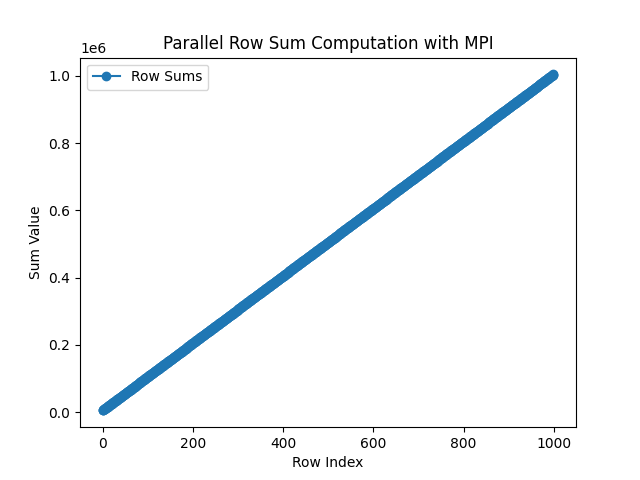
\includegraphics[width=0.9\textwidth]{img/ex2_seq}
  \caption{row summation using sequential implementation.}
  \label{fig:ex2_seq}
\end{figure}

To paralleise the code, we use \verb|MPI_Scatter(...)|.
To use MPI, we first initialise the application.

\lstinputlisting[language=C, firstline=52, lastline=56]{ex2/parallel_row_sum.c}

The main idea, is to distribute the matrix equally onto the available threads.
Our strategy is to split the matrix into chunks, each chunk contains an equal number of rows.
To achieve this, we first compute the chunk size, which is the number of rows each thread has to compute.
The basic formula for this is $\frac{N}{M}$, where $N$ is the number of rows and $M$ is the number of threads.
Because by default $N$ does not have to be divisible by $M$, we pad the matrix so that it has length $N^*$, where $N^* \mod M = 0$.
\lstinputlisting[language=C, firstline=60, lastline=61]{ex2/parallel_row_sum.c}
We initialize the matrix only on the root process and use scatter to distribute it to the rest of the threads.
This can be achieved by the following code:
\lstinputlisting[language=c, firstline=63, lastline=79]{ex2/parallel_row_sum.c}
Note, that the full matrix is only allocated on the root process!
The summation is then done on subsets of the matrix individually.
We gather all the solutions by using \verb|MPI_Gather(...)|:
\lstinputlisting[language=c, firstline=83, lastline=93]{ex2/parallel_row_sum.c}

The image looks identical to the sequential version:
\begin{figure}[H]
  \centering
  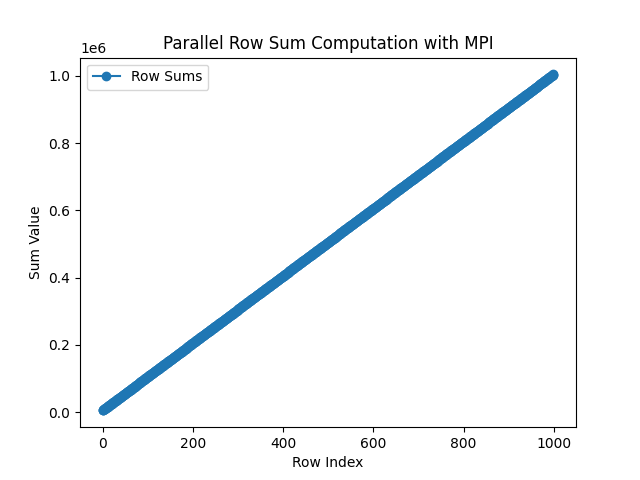
\includegraphics[width=0.9\textwidth]{img/ex2_para}
  \caption{row summation using parallel implementation.}
  \label{fig:ex2_seq}
\end{figure}

To compute the total sum, we first reduce the local result into a single local sum.
These we can then reduce globally using \verb|MPI_Reduce(...)|:
\lstinputlisting[language=c, firstline=95, lastline=102]{ex2/parallel_row_sum.c}

\todo[inline]{ex2 scaling tests...}

\section{Profiling MPI applications with Score-P and Vampir}

\section{HPC Libraries -Matrix-Vector Multiplication using BLAS}

\section{Bonus: 2D Game of Life with MPI and Non-Blocking Communication}

% content end
%###############################################################################

% \printbibliography

\end{document}
